\documentclass[lettersize,journal]{IEEEtran}
\usepackage{amsmath,amsfonts}
\usepackage{algorithmic}
\usepackage{algorithm}
\usepackage{array}
\usepackage[caption=false,font=normalsize,labelfont=sf,textfont=sf]{subfig}
\usepackage{textcomp}
\usepackage{stfloats}
\usepackage{url}
\usepackage{verbatim}
\usepackage{graphicx}
\usepackage{cite}
\hyphenation{op-tical net-works semi-conduc-tor IEEE-Xplore}
% updated with editorial comments 8/9/2021

\begin{document}

\title{Fault Tolerance Approaches\\ for Large-Scale Cloud-Based Systems}

\author{Christian Schmitz, Nico Keller, Adel Ahmadi, Raphael Pennekamp}

% The paper headers
\markboth{Report developed in the context of the masters module "Large and Cloud-based Software Systems"; As of: 8, April~2023}%
{Shell \MakeLowercase{\textit{et al.}}: A Sample Article Using IEEEtran.cls for IEEE Journals}

\maketitle
\begin{abstract}
This paper describes different approaches to increase fault tolerance in large-scale cloud-based systems. These approaches are investigated in terms of their impact for performance, cost and complexity. The goal is to find approaches and describe their constraints, implementation and impact. To investigate these approaches a prototype cloud-based system is developed and the different approaches to increase the fault tolerance are tested, measured and evaluated for this system.
\end{abstract}

\begin{IEEEkeywords}
cloud computing, reliability, fault tolerance, performance.
\end{IEEEkeywords}

\section{Introduction} 
\IEEEPARstart{I}{n}  today's fast-paced digital world, the reliability and availability of large-scale cloud-based systems are of paramount importance. These systems support numerous critical applications, ranging from social media platforms to enterprise resource planning systems, and have become an essential backbone of the modern economy. As the demand for cloud services continues to grow exponentially, so does the need for effective fault tolerance approaches to ensure the resilience and robustness of these systems. Fault tolerance is a key aspect of system design that enables the system to continue operating correctly even in the presence of component failures.\\

\noindent This research paper aims to investigate and compare the different approaches for fault tolerance in large-scale cloud-based systems, focusing on their performance, cost, and complexity. To provide a comprehensive analysis, we will develop a prototype system that incorporates various fault tolerance approaches, including hardware redundancy, software-based techniques, and hybrid solutions. This prototype will allow us to evaluate and compare the trade-offs associated with each approach in a practical setting, considering factors such as system architecture, workload, and the desired level of fault tolerance. 

\section{Research Question}

\subsection{Motivation}
\noindent As our reliance on technology continues to grow, cloud-based systems have become increasingly important for their flexibility, scalability, and cost-effectiveness. However, these systems are vulnerable to various faults and failures, including hardware failures, software bugs, and Cyberattacks. The impact of these faults can be significant, causing downtime, data loss, and damage to the service provider's reputation. This, in turn, can result in financial losses and a loss of trust from customers.
To ensure continuous availability, reliability, and data integrity, fault tolerance is crucial for cloud-based systems. Fault tolerance approaches help mitigate the effects of faults and failures, allowing the system to continue operating even in the event of a fault, while ensuring data remains consistent and accurate. 
However, implementing fault tolerance approaches involves careful consideration of their impact on system performance, cost, and complexity. Different approaches can have varying trade-offs, making it essential to carefully weigh the pros and cons of each option. Research can help identify potential trade-offs between different fault tolerance approaches in terms of performance, cost, and complexity, providing valuable insights to help make informed decisions. 
Ultimately, fault tolerance is a critical aspect of cloud-based systems. With the right approach, it's possible to ensure that these systems remain highly available, reliable, and secure, even in the face of faults and failures. By prioritizing fault tolerance, service providers can build trust with their customers, safeguarding their reputation and financial stability.

\subsection{Formulation of research question}
\noindent The primary research question for this study is: How do different approaches for fault tolerance in large-scale cloud-based systems affect performance, cost, and complexity? 
The research objectives of this report can be summarized as follows:
\begin{itemize}{}{}
\item{Investigate common approaches to increase fault tolerance in cloud-based systems.}
\item{Determine the approach with the best performance regarding the terms.}
\item{Determine the approach with the most improvement of the fault tolerance.}
\item{Compare measurable metrics and non measurable constraints and consequences.}
\item{Evaluate the of reactive approaches in terms of its trade-offs.}
\end{itemize}

\subsection{Approach}
 To research on those techniques, a prototype of a distributed system is implemented. Figure \ref{fig:fig_1} on page \pageref{fig:fig_1} shows the Use Case Diagram of the system. This system is deployed in Google Cloud. Several best practice approaches for the deployment of the system, to improve the fault tolerance of cloud-based systems are investigated. Based on their constraint matching, approaches are chosen and applied for deployment. These approaches are evaluated through the measured metrics for fault tolerance.

\begin{figure}[!t]
    \centering
    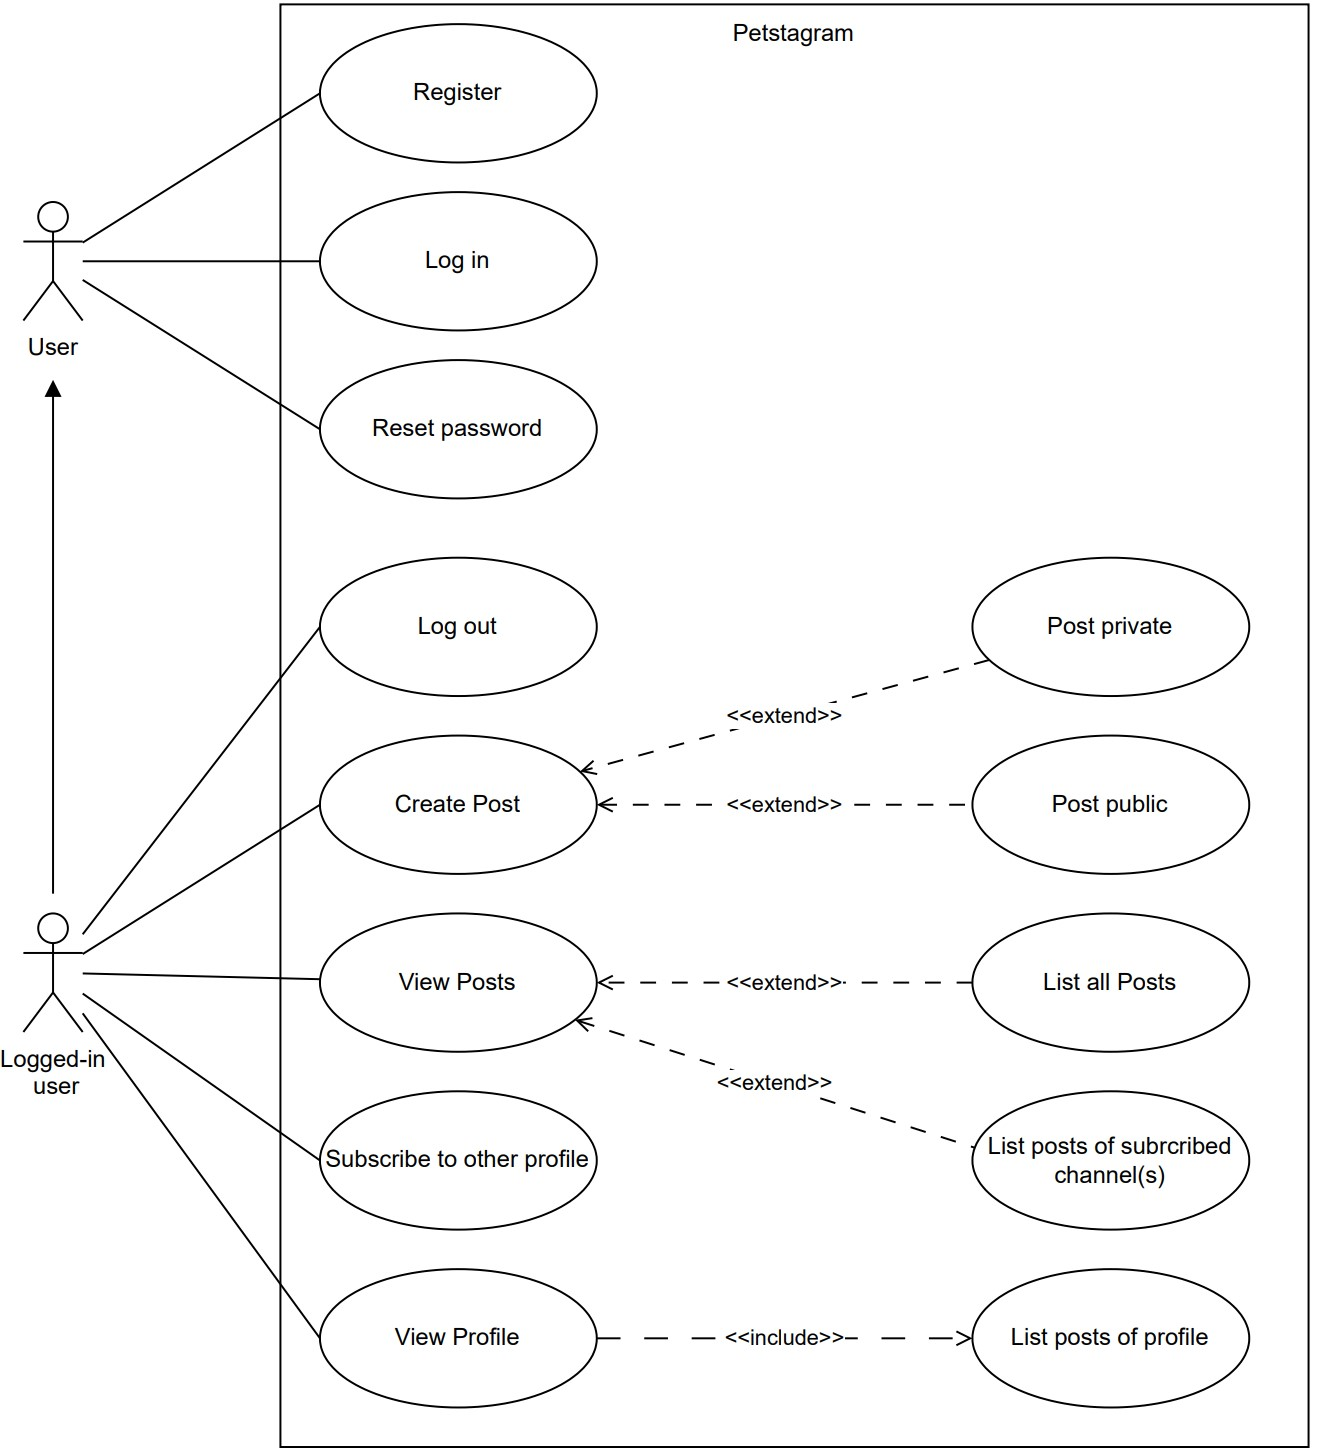
\includegraphics[width=3.5 in]{use-case-diagram}
    \caption{Use Case Diagram}
    \label{fig:fig_1}
\end{figure}

\section{Preliminary or Related Works}
\noindent 
The field of fault tolerance in cloud-based systems has been extensively studied in recent years. In this section, we provide an overview of some key research papers that have contributed to this field.

The paper "Fault-Tolerance in the Scope of Cloud Computing" \cite{paper_faultTolerance} provides a detailed understanding of fault-tolerance methods required for ensuring high availability and reliability in cloud computing environments. They highlight fault tolerance component and system-level metrics considered in cloud computing. The paper further discusses state-of-the-art proactive and reactive approaches to cloud computing fault tolerance and enumerates future research directions specific to cloud computing fault tolerance development.

Another related work is "A Survey of Fault Tolerance Architecture in Cloud Computing" \cite{paper_surveyArchitectures}. In this paper, the authors examine fault tolerance methods for cloud computing services and outline various policies and methods for implementing fault tolerance in the cloud. The paper compares various fault tolerance architectures in terms of the type of policy employed in the architecture and the method of fault detection and fault recovery.

The paper "Survey on Fault Tolerance Techniques in Cloud Computing Environment" \cite{paper_surveyTechniques} aims to provide a better understanding of various types of fault tolerance and fault tolerance techniques used in the cloud computing environment. It emphasizes the need for effective assessment and treatment of faults and presents various fault tolerance models and tools to implement them.

Lastly, the paper "Review on Fault Tolerance Techniques in Cloud Computing" \cite{paper_reviewTechniques} discusses various fault detection methods and architectural models that have been proposed to increase the fault tolerance ability of cloud computing systems. 

These related works provide valuable insights into the different approaches for fault tolerance in cloud-based systems and their impact on performance, cost, and complexity. However, there is still a need for a comprehensive analysis and evaluation of these approaches. This research paper seeks to build upon the existing knowledge base and explore the latest trends and advancements in fault tolerance strategies.

\begin{thebibliography}{1}
\bibliographystyle{IEEEtran}

\bibitem{paper_faultTolerance}
A. U. Rehman, R. L. Aguiar, and J. P. Barraca, “Fault-Tolerance in the Scope of Cloud Computing,” IEEE Access, vol. 10, 2022, doi: https://doi.org/10.1109/ACCESS.2022.3182211.
\bibitem{paper_surveyArchitectures} M. Nazari Cheraghlou, A. Khadem-Zadeh, and M. Haghparast, “A survey of fault tolerance architecture in cloud computing,” Journal of Network and Computer Applications, vol. 61, pp. 81–92, Feb. 2016, doi: https://doi.org/10.1016/j.jnca.2015.10.004.
\bibitem{paper_surveyTechniques} V. Sivagami and K. Easwarakumar, “Survey on Fault Tolerance Techniques in Cloud Computing Environment,” International Journal of Scientific Engineering and Applied Science (IJSEAS), no. 1, 2015, Accessed: Apr. 25, 2023. [Online]. Available: https://ijseas.com/volume1/v1i9/ijseas20150952.pdf
\bibitem{paper_reviewTechniques} Z. Amin, H. Singh, and N. Sethi, “Review on Fault Tolerance Techniques in Cloud Computing,” International Journal of Computer Applications, vol. 116, no. 18, pp. 11–17, Apr. 2015, doi: https://doi.org/10.5120/20435-2768.
\bibitem{paper_monolith} “Survey on Fault Tolerance Techniques in Cloud Computing Environment,” Accessed: Apr. 26, 2023. [Online]. Available: https://scaleyourapp.com/monolithic-architecture

\end{thebibliography}

\newpage

\vfill

\end{document}
